\lecture{1}{04.09.2020}{}

\section*{Análise qualitativa de sistemas dinâmicos}


Podemos aproximar um sistema em torno de um ponto de equilíbrio usando Taylor. Então sabemos que, dado um sistema $f(x)$, temos que sua derivada é \[
    f'(\overline{x}) = \lim_{x \to \overline{x}} \frac{f(x) - f(\overline{x})}{x-\overline{x}}
\] então podemos formular \[
f(x) = f(\overline{x}) + f'(\overline{x}) * (x - \overline{x})
\] que é uma aproximação linear de $f(x)$.

\begin{note}
    Dado um sistema \[
	\dot{x} = f(x) = x - x^{2}
    \] temos pontos de equilíbrio em \[
    \overline{x_1} = 0 ; \overline{x_2} = 1 
    \] então, analisando a aproximação de $f$ no equilíbrio, temos \[
    f'(\overline{x_1}) = 1 ; f'(\overline{x_2}) = -1
    \] o que implica em \[
    f_1(x) = x ; f_2(x) \sim -1*(x+1)
    \] ou seja, em torno de $\overline{x}_1$, o sistema diverge, apesar de que para $x>\overline{x}_1$ o sistema converge para $\overline{x}_2$, então não é um problema. Já em $\overline{x}_2$, o sistema converge para o ponto de equilíbrio.
\end{note}

\begin{note}
    Dado um sistema \[
	\dot{x} = f(x) = x^{2}
    \] temos um ponto de equilíbrio em $\overline{x}=0$. Mas $f'(\overline{x}) = 0$, então a aproximação linear não nos ajuda a analisar a estabilidade do sistema. Então uma análise com aproximação de segunda ordem é necessária.
\end{note}

Essa análise também é válida para sistemas de maiores dimensões \[
    \overline{x}_1 = f(x_1,x_2) ; \overline{x}_2 = f(x_1,x_2)
\] mas nesse case calculamos a Jacobiana no ponto de equilíbrio e analisamos os seus autovalores.

No caso geral, temos \[
    \dot{x} = f(x) ; x\in \R^{n}
\] definimos um ponto de equilíbrio $\overline{x}$ de tal forma que \[
f(\overline{x}) = 0
\] então aproximamos \[
\dot{x} = \overline{x} + J_f(\overline{x})(x-\overline{x})
\] em que $ J_f (\overline{x})$ é a Jacobiana de $f$ no ponto de equilíbrio. Então, se os autovalores da jacobiana são negativos, o ponto de equilíbrio é assintoticamente estável. Se são positivos, [?]. Se são mistos, é um ponto de cela, portanto instável.

Dado um sistema de controle \[
    \begin{cases}
	\dot{x}(t)=f(x,u(t)) \\
	y(t)=h(x(t))
    \end{cases}
\] com ponto de equilíbrio \[
 f(\overline{x},\overline{u})=f(0,0)=0
\] então podemos linearizar o sistema de tal forma que \[
\begin{cases}
\dot{x}(t) = Ax(t) + Bu(t) \\
y(t) = Cx(t) \\
\end{cases}
\]  onde \[
A = \frac{\partial f}{\partial x} (\overline{x},\overline{u}); B = \frac{\partial f}{\partial u} (\overline{x},\overline{u}) ; C = \frac{\partial h}{\partial x} (\overline{x})
\].

\section*{Bifurcações do Pêndulo Rotatório}

\begin{figure}[H]
    \centering
    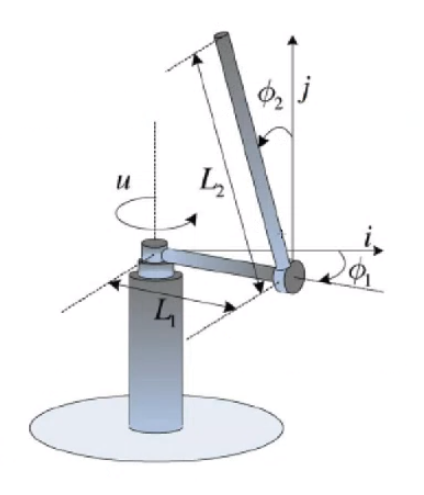
\includegraphics[width=0.6\textwidth]{figures/pendulo.png}
    \caption{Pêndulo Rotatório}
    \label{fig:figures-pendulo-png}
\end{figure}

Um pêndulo tal qual na imagem pode ser modelado como \[
\begin{cases}
    \ddot{\phi_2} - \dot{\phi_1}^{2}\sin(\phi_2)\cos(\phi_2) + \alpha\ddot{\phi_1}\cos(\phi_2) - \sin(\phi_2) + C_p \dot{\phi}_2 = 0 \\
    \ddot{\phi}_1 + C_a \dot{\phi_1} = u_a
\end{cases}
\] 

